\chapter{Factorization theorems in QCD}
In the previous chapter we have seen how, thanks to asymptotic freedom, the structure of QCD simplifies when considering problems
involving short-distance or high energy scales: the coupling becomes small and the theory can be solved perturbatively.
However, cross sections for high energy processes are usually a combination of short- and long-distance effects, and cannot
be fully computed within the framework of perturbation theory. Factorization theorems allows to separate (factorize) a cross section
or amplitude in separate contributions, each factor containing the dependence of the process on a specific distance scale:
while short-distance effects can be computed in perturbation theory, contributions coming from long-distance phenomena have
to be extracted from experimental data. 
In this chapter, starting from the Parton Model ideas we will discuss factorization theorems in QCD,
using the case of Deep Inelastic Scattering as a basic example. We will then introduce the main subject of the
present work, namely Parton Distribution Functions (PDFs).

%%%%%%%%%%%%%%%%%%%%%%%%%%%%%%%%%%%%%%%%%%%%%%%
\section{The Parton Model}
The basic ideas underlying factorization theorems for high energy processes can 
be described appealing to Feynman's parton model \cite{PhysRevLett.23.1415,Feynman:1973xc, Bjorken:1969ja}.
In this picture fundamental particles called \textit{partons} are bounded together to form hadrons.
Since the details of the partonic system are unknown, the scattering between a test particle and the hadron 
as a whole cannot be computed. However we assume that we do know how to describe the scattering with a free parton.
%
As example, let us consider the case of the scattering of a high-energy charged lepton off a
hadron target 
$$e^{-}(k)\,H\,(P)\,\rightarrow e^{-}(k')\,X \,. $$ 
Such process is known as Deep Inelastic lepton-hadron Scattering (DIS).
Looking at this scattering in the centre of mass frame, the hadron will be Lorentz contracted 
in the direction of the collision and the lifetime of the internal partonic states will be lengthened.
As a consequence, the time the electron takes to cross the hadron will be much shorter than the average lifetime of
each partonic states. During the time of the interaction the hadron can then be thought as "frozen" in 
a well defined partonic states, with each parton carrying a definite fraction $\xi$ of the hadron momentum
and not interacting with the other ones. 
If the energy of the collision is high enough, the virtual photon mediating the electron-hadron 
interaction will interact with a single parton having a given momentum fraction. Likewise, interactions
occurring in the final states are assumed to occur on time scales too long to interfere with the hard scattering.
%
Given this picture, it is natural to think about the scattering cross section as classical and incoherent,
namely as a sum of probabilities rather than of amplitudes. The parton model ideas can be summarized in the simple formula
\begin{align}
    \label{eq:parton_model}
    \sigma&\left(e^{-}\left(k\right)H\left(P\right)\rightarrow e^{-}\left(k'\right)+X\right) = \nonumber\\
     &\,\,\,\,\,\,\,\,\sum_i\int_0^1 d\xi\, q_{i/H}\left(\xi\right)
     \hat{\sigma}\left(e^{-}\left(k\right)q_i\left(\xi P\right)\rightarrow e^{-}\left(k'\right)+q_f\right)
\end{align}
where $\hat{\sigma}$ represents the partonic cross section describing the interaction between 
a single free parton and the virtual photon, and the set of functions $q_{i/H}\left(\xi\right)$ the probability densities
of having a parton of kind $i$ inside the hadron $H$, carrying a fraction $\xi \in \left(0,1\right)$ of the total hadron momentum. . 

%
In the following we recall in more details how parton model ideas apply to the case of 
DIS, setting the stage for a more complete 
discussion of factorization which will be addressed in the next section. % discussing the inclusion of NLO QCD corrections.  
DIS experiments are traditionally the main testing ground of perturbative QCD,
having been the first processes where pointlike particles were seen inside the hadron, 
thus motivating the formulation of the parton model. 
They play a central role in any discussion regarding factorization and provide a simple experimental and theoretical framework to
study the strong interaction.
As we are going to recall in the following, measurements of DIS structure functions directly probe the structure of hadrons, 
giving the bulk of experimental measurements at the basis of every phenomenological determination of Parton Distribution Functions.

\begin{figure}[h!]
    \center
    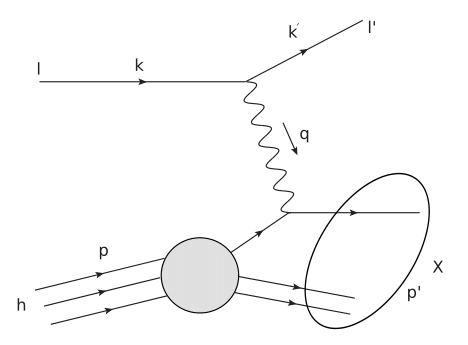
\includegraphics[scale=0.7]{dis.png}
    \caption{DIS kinematic in the parton model.}
    \label{fig:DIS_kin}
\end{figure}

The kinematic for DIS is reported in Fig.~\ref{fig:DIS_kin}.
The space-like momentum of the photon (if the initial lepton is an electron or a muon then the scattering is 
mediated by the exchange of a photon) is given by $q = k - k'$, the centre of mass energy square is $s=\left(P+k\right)^2$ and
we denote the invariant mass square of the finale states as $W = \left(P+q\right)^2$.
It is customary to introduce the kinematic variables
\begin{align}
	\label{eq:DIS_kinematic}
    & Q^2 = -q^2 > 0\,, \,\,\,\,\,\, x = \frac{Q^2}{2P\cdot q}\,, \,\,\,\,\,\, y = \frac{Q^2}{x s}\,.
    %y = \frac{P\cdot q}{P\cdot k }\,.
\end{align}
In the regime 
$$ Q^2,\, W^2 >> m^2_{\text{hadron}} \sim \Lambda^2_{\text{QCD}}\,, $$ 
leptons and quarks masses can be neglected.
It is easy to see that the variable $x$, known as \textit{Bjorken variable} can take values between 0 and 1, 
with $x\rightarrow 1$ representing the elastic limit in which $W=m^2_{\text{hadron}}$. The Deep Inelastic regime
is then defined as $Q^2 >> \Lambda^2_{\text{QCD}} $ with $x$ fixed and different from 1.

%
The corresponding amplitude reads
\begin{align}
    \label{eq:DIS_amplitude}
    \mathcal{M} = 
    \frac{e}{q^2}\bar{u}\left(k'\right)\gamma^{\alpha}u\left(k\right)\langle X | j_{\alpha}\left(0\right)|P\rangle,
\end{align}
where $|X\rangle $ represents the generic final state with $n$ on-shell particles and $j_{\alpha}$ 
is the electromagnetic current through which the photon interacts in the proton.
The cross section, which is proportional to the amplitude square, is then found to be proportional to the product between 
a leptonic and an hadronic part
\begin{align}
    \label{eq:DIS_xsec}
    \frac{d\sigma}{dx\,dQ^2} \propto \int \frac{d^3k'}{2E_{k'}\left(2\pi\right)^3}\, W^{\mu\nu}L_{\mu\nu}\,.
\end{align}
The leptonic tensor $L_{\mu\nu}$ can be easily computed within QED, while the hadronic one, containing 
the information about the interaction between the virtual photon and the hadron, can be parameterized as 
\begin{align}
    \label{eq:hadronic_tensor}
    W^{\mu\nu}\left(P,q\right) = 
    -&\left(g^{\mu\nu} -\frac{q^{\mu}q^{\nu}}{q^2}\right)F_1\left(x,Q^2\right) + \nonumber \\
    &\frac{1}{P\cdot q}\left(P^{\mu}-q^{\mu}\frac{P\cdot q}{q^2}\right)\left(P^{\nu}-q^{\nu}\frac{P\cdot q}{q^2}\right)
    F_2\left(x,Q^2\right),
\end{align}
$F_1 $ and $F_2 $ being scalar functions, called \textit{structure functions}, 
depending on the invariant quantities of the problem, namely $x$ and $Q^2$. If, more generally,
we allow $j_{\alpha}$ to be any electroweak current, there will be more than two scalar structure functions $F_i$.

%
Computing explicitly the leptonic tensor and plugging Eq.~\eqref{eq:hadronic_tensor} in Eq.~\eqref{eq:DIS_xsec} 
we can derive a general expression for the double differential cross section of DIS in the Center of Mass frame
%\begin{align}
%    \label{general cross xsec DIS}
%    \frac{d\sigma}{dx\, d} = \frac{4\pi \alpha^2}{x y Q^2}\left[xy^2F_1\left(x,Q^2\right) +\left(1-y\right)F_2\left(x,Q^2\right)\right].
%\end{align}
%or\footnote{$F_2\left(x,Q^2\right)-2 x F_1\left(x,Q^2\right) \equiv F_L\left(x,Q^2\right)$}
%\begin{align}
%    \label{general cross xsec DIS}
%    \frac{d\sigma}{dx\, dQ^2} = \frac{4\pi \alpha^2}{Q^4}\left[\left[1+\left(1-y\right)^2\right]F_1\left(x,Q^2\right) 
%    +\frac{\left(1-y\right)}{x}\left(F_2\left(x,Q^2\right)-2 x F_1\left(x,Q^2\right)\right)\right].
%\end{align} 

\begin{align}
    \label{general cross xsec DIS}
    \frac{d\sigma}{dx\, dQ^2} = \frac{2\pi \alpha^2}{Q^4}\left[\left[1+\left(1-y\right)^2\right]F_T\left(x,Q^2\right) 
    +\frac{2\left(1-y\right)}{x}F_L\left(x,Q^2\right)\right]\,,
\end{align}
where $\alpha = e^2/\left(4\pi\right)$ is the fine structure constant and the transverse and longitudinal structure functions 
are defined as
\begin{align}
    F_L = F_2 -2F_1\,, \,\,\,\, F_T = 2F_1\,.
\end{align}
%Following the same steps, considering a single parton of momentu $\xi P$ in the initial state,
%we can introduce partonic structure functions $\hat{F}_1$, $\hat{F}_2$ to parameterized the 
%parton level cross section $\hat{d\sigma}$ for the lepton-parton scattering.

%
The partonic cross section $d\hat{\sigma}$ for the scattering of the lepton off a single parton with momentum $\xi P$
can be computed through a simple leading order QED computation ($e^- + q \rightarrow e^- + q $) getting
\begin{align}
    \frac{d\hat{\sigma}}{dx\, dQ^2} = 
    \frac{4\pi \alpha^2}{Q^4}\left[1+\left(1-y\right)^2\right]\frac{1}{2} e^2\delta\left(x-\xi\right)\,,
\end{align}
from which we can read the expressions for the partonic structure functions 
$\hat{F}_1$ and $\hat{F}_2$
\begin{align}
    \hat{F}_2 = x e^2 \delta\left(x-\xi\right) = 2x \hat{F}_1\,.
\end{align}
%
Finally, using the parton model assumption of Eq.~\eqref{eq:parton_model}, we can write
an explicit expression for the full structure functions
%\begin{align}
%    \label{structure functions}
%    F_i\left(x,Q^2\right)= \int_x^1\frac{d\xi}{\xi}\sum_j f_j\left(\xi\right)\hat{F}_{ij}\left(\frac{x}{\xi},Q^2\right)
%\end{align}
%where $F_i = F_1, \, F_2/x $, so that

\begin{align}
    \label{eq:LO DIS xsex}
    &F_L\left(x,Q^2\right) = 0\,,\,\,\,\,\,\, 
    F_2\left(x,Q^2\right) = x\sum_a e_a^2\, q_{a/H}\left(x\right)\,. 
    %&\frac{d\sigma}{dx\,dQ^2} = \frac{2\pi\alpha^2 s}{Q^4}\left(\sum_f x f_f\left(x\right)Q_f^2\right)\left[1+\left(1-y\right)^2\right]\,.
\end{align} 
Eq.~\ref{eq:LO DIS xsex} makes manifest how DIS experiments probe the structure of the incoming hadron $H$,
giving direct access to the functions $q_{a/H}\left(x\right) $ encoding its internal distribution of quarks and gluons.
Also, it shows explicitly how in the parton model the structure functions do not depend on the energy scale.
Such property is known as Bjorken scaling, and its experimental observation was taken as a confirmation
of the composite nature of hadrons, confirming the picture of the parton model.

\comment{some final remark about parton model, maybe smt about sum rules and the evidence for the 
presence of the gluon, references.}

%%%%%%%%%%%%%%%%%%%%%%%%%%%%%%%%%%%%%%%%%%%%%%%%%%%%
\section{Improved Parton Model and factorization of collinear singularities}
In this section, starting from the parton model ideas, we briefly recall how to include Next-to-Leading-Order
(NLO) QCD corrections.
As we are going to see, when considering QCD corrections two important things happen.
First Bjorken scaling is broken, namely the structure functions acquire a non trivial scale dependence.
Second, when considering gluons emissions from the initial state particles, infrared collinear singularities
arise. The universal factorization of such collinear poles and the subsequent renormalization of parton distribution functions
represent the main conceptual point of factorization in high energy processes, and 
will be discussed in the following.  

%
\subsection{Next-to-Leading-Order QCD corrections}
Considering a generic structure function $F$, following the parton model ideas we can write it as
\begin{align}
    \label{eq:strcuture_function}
    F\left(x,Q^2\right) = \sum_a \int_x^1 \frac{d\xi}{\xi}\, q^{\bare}_{a/H}\left(\xi\right)\, \hat{F}_a\left(\frac{x}{\xi},Q^2\right)\,,
\end{align}
with $\hat{F}_a$ representing the partonic level structure function for the scattering of a
quark off the virtual photon, and $q^{\bare}_{a/H}$ denoting the parton model PDFs
\footnote{Although here we are introducing this formula starting from the ideas of the parton model, 
Eq.~\eqref{eq:strcuture_function} can be proved in the Bjorken limit, and the bare PDF $q^{\bare}_{a/H}$ can be
defined in terms of a bilocal operator matrix element. We will get back to this point in the next sections}. 
Such formula is valid at leading-twist, namely further corrections of non-pertubative origin are suppressed by powers
of $\Lambda_{QCD}/Q$.

%
From the previous section we know that at Born level $\hat{F}_a$ is proportional
to a delta function $e^2\delta\left(1-x\right)$. 
Considering QCD correction of order $\alpha_s$
initial and final states emissions of a single gluon, corresponding to Feynman diagrams of Fig.~\ref{fig:NLO_QCD_DIS}
have to be computed. 
Accounting also for the corresponding virtual corrections on the quark legs
and for the gluon induced vertex correction, the full result has the following form
\begin{align}
    \label{eq:1_loop_dis}
    \hat{F}\left(x,Q^2\right) = e^2\left[\delta\left(1-x\right) 
    + \alpha_s\left(P\left(x\right)\log\frac{Q^2}{Q_0^2} + R\left(x\right) \right)  \right]\,,
\end{align}
with
\begin{align}
    \label{eq:splitting_function}
    P\left(x\right) = \frac{C_F}{2\pi}\left[\frac{1+x^2}{\left(1-x\right)_+} + \frac{3}{2}\delta\left(1-x\right)\right]\,.
\end{align}
Two observations can be done. Firstly, as anticipated above, beyond leading order
Bjorken scaling is broken by logarithms of $Q^2$, and the structure function acquires a $Q^2$ dependence.
Secondly, Eq.~\ref{eq:1_loop_dis} contains a logarithmic dependence on an infrared cutoff $Q_0^2$, pointing out 
the presence of an infrared divergence.
\begin{figure}[h]
    \centering
    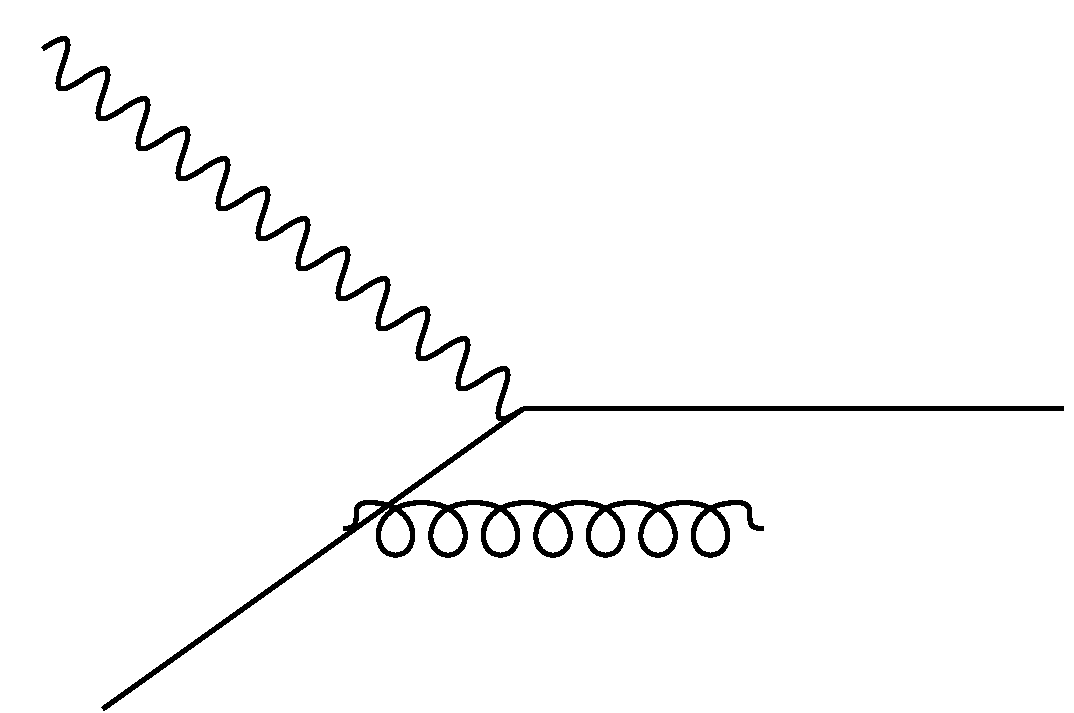
\includegraphics[scale=0.2]{real_initial_DIS.pdf}
    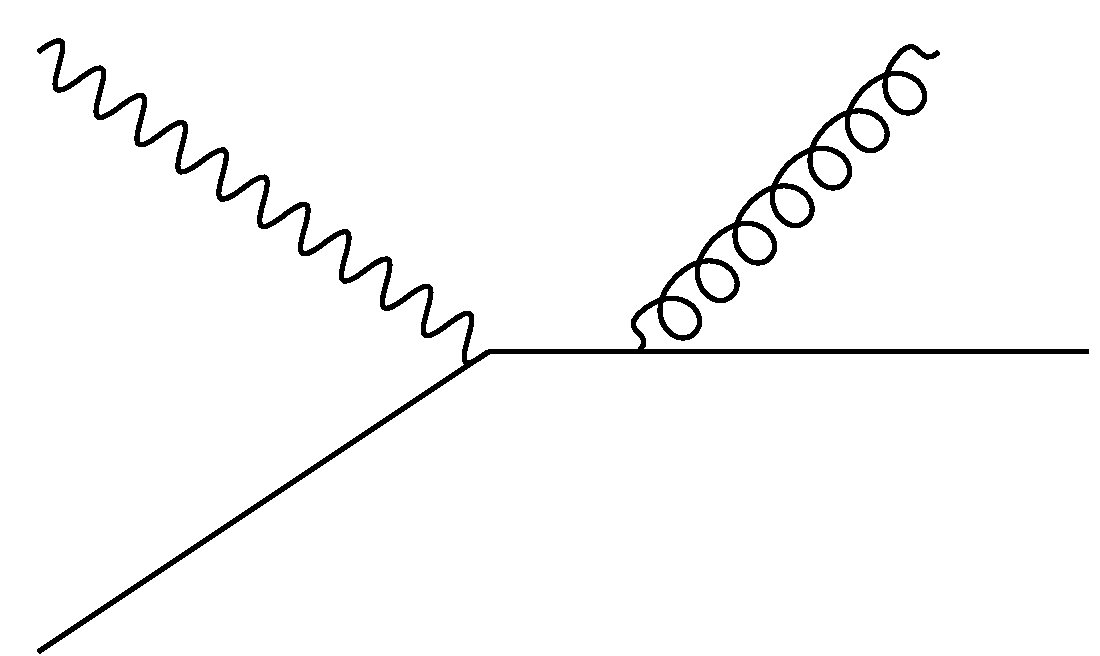
\includegraphics[scale=0.2]{real_final_DIS.pdf}
    \caption{Real NLO QCD corrections.}
    \label{fig:NLO_QCD_DIS}
\end{figure}

%
Working in a light-cone gauge, such logarithmic divergence can be traced back to the square of the amplitude associated
to a gluon emission from the initial state quark.
It can be shown, that denoting as $k_{\perp}$ the longitudinal momentum of the emitted gluon,
we end up with a contribution of the form
\begin{align}
    \label{eq:collinear_div}
    \hat{F}_{q\, \gamma \rightarrow q\,g}\left(x,Q^2\right) =
    \int^{\,Q^2}\frac{dk_{\perp}^2}{k_{\perp}^2}\, \alpha_s\, P\left(x\right) + ...\,,
    %\sim \alpha_s\left(Q^2\right)\,\log\frac{Q^2}{Q_0^2}\,,
\end{align}
where the ellipses stand for finite regular terms.
It is clear from Eq.~\ref{eq:collinear_div} that such term diverges in the region of small-$k_{\perp}$.
In order to regularize such pole we can introduce the infrared cutoff $Q_0^2$, getting the logarithmic 
contribution observed in Eq.~\ref{eq:1_loop_dis}.
Similarly, when considering multiple gluons emissions from initial state particles, terms of the kind 
$\left(\alpha_s\left(Q^2\right)\,\log\frac{Q^2}{Q_0^2}\right)^n$ show up.
Since all these terms are of order 1, if we accounted for only some of them we would spoil perturbation theory.
In order to get a proper perturbative expansion such terms have to be resummed at all orders.
Such resummation is achieved through factorization of collinear singularities into the parton model PDFs,
as described in the next section.

\subsection{Factorization of collinear singularities}
The singularities described in the previous sections arises from the kinematic region where $k_{\perp}\rightarrow 0$,
namely when a gluon is emitted parallel to an initial state quark. For this reason they are often called collinear
singularities.
To understand how to deal with such terms, one needs to realize that the limit of small$-k_{\perp}$
corresponds to the long-range (low energy) regime of the strong interaction and therefore cannot be treated
within perturbation theory.
We can then consider the parton distributions introduced through the parton model as bare, unmeasurable
quantities, and use them to reabsorb the collinear singularities. In this way, all the dependence on
low energy phenomena can be factorized in the parton distribution functions, leaving the hard
cross sections free from collinear singularities.

%
Starting from the logarithmic divergent contribution appearing in Eq.~\eqref{eq:1_loop_dis}, we can introduce an
additional unphysical scale $\mu_F$ and write
$\log\frac{Q^2}{Q_0^2} = \log\frac{Q^2}{\mu_F^2} + \log\frac{\mu_F^2}{Q_0^2} $.
Looking back at Eq.~\eqref{eq:strcuture_function},
the infrared divergent partonic structure function can then be written as
\begin{align}
  \label{eq::IRsubtraction}
  \hat{F}\left(\xi,Q\right) = 
  \int_{\xi}^1 \frac{d\eta}{\eta} \,\Gamma\left(\frac{\xi}{\eta},\mu_F\right)
  \hat{F}_{\text{reg}}\left(\eta,\frac{Q}{\mu_F}\right) ,
\end{align}
with
\begin{align}
    &\Gamma\left(y,\mu_F\right) = \delta\left(1-y\right) 
    + \alpha_s\left[P\left(y\right)\log\frac{\mu_F^2}{Q_0^2} + \Gamma_{finite}\left(y\right)\right]\,, \\
    &\hat{F}_{\text{reg}}\left(\eta,\frac{Q}{\mu_F}\right) = \delta\left(1-\eta\right)  
    + \alpha_s
    \left[P\left(\eta\right)\log\frac{Q^2}{\mu_F^2}+ R\left(\eta\right) - \Gamma_{finite}\left(\eta\right) \right]\,.  
\end{align}
The new scale $\mu_F$ introduced above, often referred to as factorization scale, separates long and short distance 
contributions: everything which is below $\mu_F$ is considered to be in a non perturbative regime 
and it is factorized in the kernel $\Gamma$, which therefore contains the infrared poles.
The term $\Gamma_{finite}$ represents finite contributions that can be
kept into the subtraction kernel rather than in the hard structure function. Its specific choice is what defines
the renormalization scheme.  
Substituting Eq.~\eqref{eq::IRsubtraction} in Eq.~\eqref{eq:strcuture_function} it is easy to see that
we can write
\begin{align}
  F\left(x,Q\right) = \sum_a\int_x^1 \frac{d\eta}{\eta}\, 
  q_{a/H}\left(\eta,\mu_F\right)\hat{F}_{\text{reg}}\left(\frac{x}{\eta},\frac{Q}{\mu_F}\right),
\end{align}
where the renormalized quark PDFs $q_{a/H}$ is defined as
\begin{align}
    \label{eq:renormalized_pdf}
    q_{a/H}\left(x,\mu_F\right) = \int_x^1 \frac{d\eta}{\eta} \,
    q^{\bare}_{a/H}\left(\frac{x}{\eta}\right)\Gamma\left(\eta, \mu_F\right)\,.
\end{align}
Collinear poles are therefore factorized from the hard scattering structure function and reabsorbed into
the PDFs, following a procedure symilar to the one used for UV renormalization.
As a consequence PDFs acquire a non trivial dependence on an unphysical scale $\mu_F$,
which will be further described in in the next section.

%
To sum up, considering higher orders QCD corrections, the DIS structure functions can be written
as
\begin{align}
    \label{eq:dis_qcd}
    F\left(x,Q^2\right) = 
    \sum_a \int_x^1\frac{d\xi}{\xi}\,C_a\left(\frac{x}{\xi},\frac{Q^2}{\mu_F^2}, \alpha_s\right)q_{a/H}\left(\xi,\mu_F^2\right)
    +\mathcal{O}\left(\frac{\Lambda_{QCD}}{Q}\right)\,.
\end{align}
The coefficients functions $C_a$ appearing in Eq.~\eqref{eq:dis_qcd} correspond to the finite partonic structure 
functions $\hat{F}_{\text{reg}}$ after renormalization and subtraction of collinear singularities.
Their explicit expression will depend on the specific structure function under consideration
and on the choice for the renormalization and factorization schemes, defined when removing UV and collinear
singularities respectively. 
Once properly defined they can be computed order by order in perturbation theory as an expansion in the strong coupling
\begin{align}
    \label{eq:coeff_functions_expansion}
    C_a\left(x, \alpha_s\right) = C_a^{(0)}\left(x\right) + \alpha_s\, C_a^{(1)}\left(x\right) 
    + \alpha_s^2\, C_a^{(2)}\left(x\right) + ...\,,
\end{align}
where the first contribution (LO) recover the parton model predictions, the second one (NLO) corresponds to the QCD
corrections discussed above and the coming ones (N$^{\text{n}}$NLO) will refer to higher order corrections.
Differently from the initial formula of Eq.~\eqref{eq:strcuture_function}, which was written in analogy to
the parton model formulation, the parton distributions
have now acquired a scale dependence, which cancel against an analogue dependence in the coefficient functions,
leaving the physical structure function independent from any unphysical scales. Also, even if in our 
discussion we have only considered the quark channel, the sum over the flavour types $a$ now includes
also gluon initiated contributions, which formally start at NNLO.

%
So far we have discussed factorization for processes with only one hadron in the initial state, but
the same ideas and logic apply to inclusive enough high-energy hadron-hadron collisions
$$
H_1\left(p_1\right) + H_2\left(p_2\right) \rightarrow W\left(Q\right) + X\,,
$$
where $H_1$ and $H_2$ are the incoming hadrons, having momenta $p_1$ and $p_2$, $H$ represents
the particle produced in the hard scattering (Higgs or vector bosons, heavy quarks) and $W$
denotes any other particle appearing in the final state. In this case the factorization formula takes the form
\begin{align}
    \label{eq:hadron_hadron}
    \sigma&\left(p_1,p_2,Q\right) = \sum_{a,b}\int_{\tau}^1\, 
    dx_1 dx_2 \, \nonumber \\ 
    &q_{a/H_1}\left(x_1,\mu_F^2\right)q_{b/H_2}\left(x_2,\mu_F^2\right)
    \hat{\sigma}_{ab}\left(x_1p_1,x_2p_2,\frac{Q^2}{\mu_F^2},\alpha_s\right) 
    + \mathcal{O}\left(\frac{\Lambda_{QCD}}{Q}\right)\,,
\end{align}
where $\tau = \frac{Q^2}{s}$ and $s=\left(p_1+p_2\right)^2$.

%
The two factorized expressions given in Eqs.~\eqref{eq:dis_qcd},~\eqref{eq:hadron_hadron}
allow to connect cross sections for high-energy processes having hadrons in the initial states to hard scattering processes.
The former can be measured in collider experiments, while the latter 
can be computed in perturbation theory. The objects connecting perturbation theory with physical observables are
the Parton Distribution Functions.
The content of the factorization theorem is that all the dependence
on low mass phenomena is entirely contained in the PDFs. Therefore, since they describe the internal structure 
of a given kind of hadron and have been decoupled from the short-distance details of
the specific process we consider, they are nonpertubative and universal objects.
This means that the PDFs appearing in the case of DIS must be the same considered for 
any other high-energy collisions.

%%%%%%%%%%%%%%%%%%%%%%%%%%%%%%%%%%%%%%%%%%%%%%%%%%%%
\section{Parton Distribution Functions}
In the previous section we have introduced PDFs as some bare objects,
which are then used to reabsorb the infrared collinear poles coming from the fixed order computation of partonic
hard cross sections. Following this approach PDFs are introduced in the discussion through 
the parton model ideas, and defined as objects containing all the dependence 
of the physical observable on low energy physics. 
%
It is possible to give a rigorous operator definition of parton distributions,
which can be applied beyond perturbation theory and makes manifest the universal nature of PDFs.
The formalism and notations commonly used to describe PDFs in terms of QCD operators are usually quite different
from those introduced in the previous section, which are commonly adopted for phenomenological applications.
Since in this work we will present results for which both formalism are required,
in this section we briefly revise the formal definition of PDFs, addressing their UV renormalization
and renormalization group equation and making contact with the formalism and notations introduced in the previous section.

\subsection{PDFs operator definition}
Working in the Bjorken limit, it can be proved~\cite{Collins:1980ui,Collins:1981uw} that the bare unpolarized 
quark PDF appearing in Eq.~\eqref{eq:strcuture_function} is related to the light-cone Fourier transform 
of a bilocal operator, given by
\begin{align}
	\label{eq::barepdf}                                                  
	f_\mathrm{q}^\bare\lp x \rp = \int \frac{d\xi^-}{4\pi} e^{-ixP^+\xi^-} 
	\langle \text{P}|\bar{\psi}_\mathrm{q}^\bare\lp\xi^-\rp\gamma^+ \,   
	U\lp\xi^-,0\rp \psi_\mathrm{q}^\bare\lp 0\rp  |\text{P}\rangle\, ,   
\end{align}
where $|\text{P}\rangle$ denotes a hadronic state with momentum $P^\mu = \lp
P^0,0,0,P^z\rp$, $x$ belongs to the real interval $\left[-1,1\right]$ and $P^{\pm}=\frac {\lp P^0 \pm P^z \rp}{ \sqrt{2}}$ are
light-cone coordinates. 
The index $\mathrm{q}$ identifies the parton under
investigation. For instance, in a theory where we only consider the four
lightest quarks, we have $q=u,d,s,c$. The momentum carried by the parton is
$k^\mu = x P^\mu$, $\psi_\mathrm{q}^\bare$ is the bare quark field operator and the
Wilson line $U$ is given by 
\begin{align}
	\label{eq::wilsonline}                                                      U\lp\xi^-,0\rp = \text{P}\exp 
    \lp -ig\int_0^{\xi^-}d\eta^- A^{\bare\,+}\lp \eta^- \rp \rp\, .         
\end{align}
An analogous definition can be given for the gluon bare PDFs, denoted as
$f_g^\bare\lp x \rp$. The superscripts $\bare$ in the above expressions identify
bare fields: the matrix elements that enter in the definition of
$f_\mathrm{q}^\bare$ are ultraviolet divergent, and therefore need to be
renormalized.
Renormalized parton distributions are usually defined by minimal
subtraction, and the relation between the bare and the renormalized quantities
is given by
\begin{align}
	\label{eq:RenormPDF}                                   
	f_a^\bare\lp x \rp = \sum_{b}\int_x^1\frac{dy}{y}\,\text{Z}_{ab}\lp\frac{x}{y},\mu \rp f_b\lp y,\mu^2 \rp\, , 
\end{align}
where the indices $a$ and $b$ run over all the parton types (gluon and flavors
of quarks) and $\mu$ denotes the renormalization scale introduced by the minimal
subtraction scheme. 

Focusing on the quark PDFs for now, the renormalized distributions introduced
above have a compact support given by the interval $[-1,1]$. 
To recover the conventions of the previous sections, used for
phenomenological applications, it is customary to define the PDFs on the
interval $[0,1]$, and to introduce independent functions for the quarks and the
antiquarks, which we have previously denoted as $q(x,\mu^2)$ and $\bar{q}(x,\mu^2)$ respectively.
The relation between $f_q$, $q$ and $\bar{q}$ is 
\begin{equation}
    \label{eq:DefFQQbar}
    f_\mathrm{q}\lp x,\mu^2\rp = 
    \begin{cases}
        \phantom{-}q(x,\mu^2)\, , &\quad \mathrm{if}\ x>0\, , \\
        -\bar{q}(-x,\mu^2)\, , &\quad \mathrm{if}\ x<0 \, .
    \end{cases}
\end{equation}
It is useful to consider the symmetrised and antisymmetrised combinations of
$f_\mathrm{q}$ in the interval $x\in[0,1]$:
\begin{eqnarray}
	\label{eq:fsym}
	f^\mathrm{sym}_\mathrm{q}(x,\mu^2)  &= f_\mathrm{q}(x,\mu^2) + f_\mathrm{q}(-x,\mu^2) 
	\, , \\
	\label{eq:fasym}
	f^\mathrm{asy}_\mathrm{q}(x,\mu^2)  &= f_\mathrm{q}(x,\mu^2) - f_\mathrm{q}(-x,\mu^2) \, .
\end{eqnarray}
It can be readily shown that
\begin{align}
    f^\sym_\mathrm{q}(x,\mu^2) &= 
    q(x,\mu^2) - \bar{q}(x,\mu^2) = q^-(x,\mu^2) \, , \\
    f^\asy_\mathrm{q}(x,\mu^2) &= 
    q(x,\mu^2) + \bar{q}(x,\mu^2) = q^+(x,\mu^2) \, .
\end{align}
where $q^+$ and $q^-$ are defined by the equations above. The flavor
decomposition can be rewritten by collecting the quark fields in a vector, \eg\
$\psi = \lp \psi_u,\psi_d,\psi_s,\psi_c\rp$, and defining the following nonsinglet bare
PDFs:
% \begin{eqnarray}
%     \label{eq:f3Def}
%     f_3^\bare(x) &= \int \frac{d\xi^-}{4\pi} e^{-ixP^+\xi^-} 
% 	\langle \text{P}|\bar{\psi}^\bare\lp\xi^-\rp \lambda_3 \gamma^+ \,   
% 	U\lp\xi^-,0\rp \psi^\bare\lp 0\rp  |\text{P}\rangle\, ,  \\
%     \label{eq:f8Def}
%     f_8^\bare(x) &= \int \frac{d\xi^-}{4\pi} e^{-ixP^+\xi^-} 
% 	\langle \text{P}|\bar{\psi}^\bare\lp\xi^-\rp \lambda_8 \gamma^+ \,   
% 	U\lp\xi^-,0\rp \psi^\bare\lp 0\rp  |\text{P}\rangle\, ,  \\
%     \label{eq:f15Def}
%     f_{15}^\bare(x) &= \int \frac{d\xi^-}{4\pi} e^{-ixP^+\xi^-} 
% 	\langle \text{P}|\bar{\psi}^\bare\lp\xi^-\rp \lambda_{15} \gamma^+ \,   
% 	U\lp\xi^-,0\rp \psi^\bare\lp 0\rp  |\text{P}\rangle\, ,  
% \end{eqnarray}
\begin{eqnarray}
    \label{eq:fADef}
    f_A^\bare(x) &= \int \frac{d\xi^-}{4\pi} e^{-ixP^+\xi^-} 
	\langle \text{P}|\bar{\psi}^\bare\lp\xi^-\rp \lambda_A \gamma^+ \,   
	U\lp\xi^-,0\rp \psi^\bare\lp 0\rp  |\text{P}\rangle\, , 
\end{eqnarray}
where $A=3,8,15$, and we have used the Gell-Mann matrices
\begin{eqnarray}
    \lambda_3=
    \begin{pmatrix}
        1 & 0 & 0 & 0\\
        0 & -1& 0 & 0\\
        0 & 0 & 0 & 0\\
        0 & 0 & 0 & 0
    \end{pmatrix}\, , \quad
    \lambda_8=
    \begin{pmatrix}
        1 & 0 & 0 & 0\\
        0 & 1& 0 & 0\\
        0 & 0 & -2 & 0\\
        0 & 0 & 0 & 0
    \end{pmatrix}\, , \quad
    \lambda_{15}=
    \begin{pmatrix}
        1 & 0 & 0 & 0\\
        0 & 1& 0 & 0\\
        0 & 0 & 1 & 0\\
        0 & 0 & 0 & -3
    \end{pmatrix}\, . 
\end{eqnarray}
In this notation $f_3$ corresponds to $f^{u-d}=f_u-f_d$, $f_8=f^{u+d-2s}$, and
so on. The symmetrised and antisymmetrised combinations map directly into the
so-called {\em evolution basis} for the PDFs that is normally used in
phenomenological studies, see \eg\ Ref.~\cite{Vogt:2004ns} for a detailed
definition of the flavor decomposition. More specifically, we have:
\begin{align}
    f^\asy_{3}  &= u^+ - d^+ = T_3 \, , \\
    f^\sym_{3}  &= u^- - d^- = V_3 \, , \\
    f^\asy_{8}  &= u^+ + d^+ - 2 s^+ = T_8 \, , \\
    f^\sym_{8}  &= u^- + d^- - 2 s^- = V_8 \, , \\
    f^\asy_{15} &= u^+ + d^+ + s^+ - 3 c^+ = T_{15} \, , \\
    f^\sym_{15} &= u^- + d^- + s^- - 3 c^- = V_{15} \, .
\end{align}

%
As mentioned above the bilocal operator products of Eq.~\ref{eq::barepdf} requires renormalization.
The corresponding renormalization group equations are the Altarelli-Parisi equations fo PDFs.
Considering on-shell incoming partons, a straightforward 1-loop computation gives
\begin{align}
    \label{eq:1-loop_bare_partonic_pdf}
    f^{\bare}_{a/b}\left(x,\epsilon\right) = \delta_{ab}\,\delta\left(1-x\right)
    + \alpha_s\left[\frac{1}{\epsilon_{UV}}-\frac{1}{\epsilon_{IR}}\right] P_{a/b}^{(1)}\left(x\right)
    + \mathcal{O}\left(\alpha_s^2\right)\,.
\end{align}
To obtain such result, one has to work in dimensional regularization to regularize both UV and infrared
divergences. 
Working in $\overline{MS}$ the UV pole $1/\epsilon_{UV}$ is removed through renormalization,
and we are left with the renormalized partonic PDFs
\begin{align}
    \label{eq:1-loop_renormalized_partonic_pdf}
    f_{a/b}\left(x,\epsilon\right) = \delta_{ab}\,\delta\left(1-x\right)
    + \alpha_s\left(-\frac{1}{\epsilon}\right) P_{a/b}^{(1)}\left(x\right)
    + \mathcal{O}\left(\alpha_s^2\right)\,.
\end{align}
Such object, despite being UV finite, does contain 
infrared poles.

%
We can now see how the formal approach followed here recovers the picture given in the previous section.
Taking as example the case of DIS structure function, we can apply Eq.~\ref{eq:dis_qcd} to the case of an 
incoming parton $b$\footnote{An important property of the hard coefficient functions is that they 
depend only on the parton type $a$ and not on the specific hadron $H$, 
so that they can be computed with the simplest choice of external parton.}
\begin{align}
    \label{eq:partonic_structure_function}
    \hat{F}_{b}\left(x,\epsilon\right) = 
    \sum_a \int_x^1\frac{d\xi}{\xi}\,C_a\left(\frac{x}{\xi}, \alpha_s\right)f_{a/b}\left(\xi,\epsilon\right)
    +\mathcal{O}\left(\frac{\Lambda_{QCD}}{Q}\right)\,.
\end{align}
Considering the coefficient functions power expansions given in Eq.~\eqref{eq:coeff_functions_expansion}
and an analogue expansion for $\hat{F}_{a}$, using the 1-loop expression for the
renormalized partonic PDF of Eq.~\eqref{eq:1-loop_renormalized_partonic_pdf} we get
\begin{align}
    \label{eq:IR_subtraction_from_formal_definition}
    &C^{(0)}_b\left(x\right) = \hat{F}_b^{(0)}\left(x\right)\,,\\
    &C^{(1)}_b\left(x\right) = \hat{F}_b^{(1)}\left(x,\epsilon\right) + \frac{1}{\epsilon}\sum_a\int_x^1 \frac{d\xi}{\xi}P_{a/b}^{(1)}\left(\xi\right)
    \hat{F}_a^{(0)}\left(\frac{x}{\xi}\right)\,,
\end{align}
which recovers the prescription introduced in the previous section: in order to compute
the hard scattering cross sections, one should calculate the structure function at the parton level and subtract
from it certain infrared divergent terms proportional to the splitting kernel and the Born cross section.
Such terms, identified as collinear emissions in the previous sections, here are computed in a process independent
way starting directly from the formal definition of PDFs.
Another way of stating this, is that the infrared subtraction kernel $\Gamma$ introduced in Eq.~\eqref{eq::IRsubtraction}
corresponds to the parton level renormalized PDF of Eq.~\eqref{eq:1-loop_renormalized_partonic_pdf}. For a proof
of this at every order in perturbation theory see for example \cite{Collins:1980ui}.


\subsection{DGLAP evolution equations}
\label{sec:DGLAP}
As stated in Eq.~\ref{eq:RenormPDF} the operator defining parton distribution functions requires
renormalization. As a consequence renormalized PDFs acquire a scale dependence.
Including in the discussion also the gluon PDF, the corresponding renormalization group equations read
\begin{align}
    \mu^2\frac{\partial}{\partial\mu^2}
    \begin{pmatrix}
        q_i\left(x,\mu^2\right) \\  
        g\left(x,\mu^2\right)
    \end{pmatrix}
    =
    \alpha_s\sum_{q_i,\bar{q}_i}\int_x^1 \frac{d\xi}{\xi} 
    \begin{pmatrix}
        P_{q_i q_j}\left(\frac{x}{\xi},\alpha_s\right) & P_{q_i g}\left(\frac{x}{\xi},\alpha_s\right) \\
        P_{g q_j}\left(\frac{x}{\xi},\alpha_s\right)   & P_{g g}\left(\frac{x}{\xi},\alpha_s\right) 
    \end{pmatrix}
    \begin{pmatrix}
        q_j\left(x,\mu^2\right) \\  
        g\left(x,\mu^2\right)
    \end{pmatrix}
\end{align}
with each splitting function computable in perturbation theory
\begin{equation}
    \begin{split}
    &P_{q_i q_j}\left(x,\alpha_s\right) = \delta_{ij}P^{(0)}_{qq}\left(x\right) 
    + \alpha_s P^{(1)}_{q_i q_j}\left(x\right) + ... \\
    &P_{q g}\left(x,\alpha_s\right) = P^{(0)}_{qg}\left(x\right) 
    + \alpha_s P^{(1)}_{q g}\left(x\right) + ... \\
    &P_{g q}\left(x,\alpha_s\right) = P^{(0)}_{gq}\left(x\right) 
    + \alpha_s P^{(1)}_{gq}\left(x\right) + ... \\
    &P_{g g}\left(x,\alpha_s\right) = P^{(0)}_{gg}\left(x\right) 
    + \alpha_s P^{(1)}_{gg}\left(x\right) + ... 
    \end{split}
\end{equation}
It is convenient to re-express the DGLAP equations choosing a PDFs basis which maximally diagonalize them. 
In order to do this the aforementioned evolution basis is particularly useful.
Denoting 
\begin{align}
    q^{\pm}_i = q_i \pm \bar{q}_i\,,
\end{align}
and considering the flavours $u, d, s, c, b, t$ the non-singlet sector is defined by the valence distributions
\begin{align}
    V_i = q_i^-
\end{align} 
and the $T_i$ combinations, defined as
\begin{align}
    T_3 = u^+ - d^+\,,\,\,\,\,\,\,T_8 = u^+ + d^+ -2s^+\,,\,\,\,\,\,\,T_{15} = u^+ + d^+ + s^+ -3c^+\,,\,\,\,\,\,\, \\
    T_{24} = u^+ + d^+ + s^+ + c^+ -4b^+\,,\,\,\,\,\,\, T_{35} = u^+ + d^+ + s^+ + c^+ + b^+ - 5 t^+\,. 
\end{align}
Each non-singlet distribution will then satisfy an independent evolution equation, given by 
\begin{align}
    \label{eq:DGLAP_NS}
    \mu^2\frac{d}{d\mu^2}q^{NS}\left(x,\mu^2\right) 
    = \int_{\xi}^1\frac{d\xi}{\xi}P\left(\xi,\alpha_s\right)
    q^{NS}\left(\frac{x}{\xi},\mu^2\right)\,.
\end{align}
The spitting function $P$ for $V_i$ and $T_i$ distributions is given by $P^-$ and $P^+$ respectively,
which at leading order are
\begin{align}
    P^{-(0)}\left(x\right) = P^{+(0)}\left(x\right) = \frac{C_F}{2\pi}\left(\frac{1+z^2}{1-z}\right)_+ \,.
\end{align}
Working in the evolution basis, the only distribution which couples to the gluon is the so called
singlet combination, defined as
\begin{align}
    \Sigma\left(x,\mu^2\right) = \sum_i \left(q_i\left(x,\mu^2\right)+\bar{q}_i\left(x,\mu^2\right)\right)
\end{align}
\begin{align}
    \mu^2\frac{\partial}{\partial\mu^2}
    \begin{pmatrix}
        \Sigma\left(x,\mu^2\right) \\  
        g\left(x,\mu^2\right)
    \end{pmatrix}
    =
    \alpha_s\int_x^1 \frac{d\xi}{\xi} 
    \begin{pmatrix}
        P_{q q}\left(\frac{x}{\xi},\alpha_s\right) & P_{q g}\left(\frac{x}{\xi},\alpha_s\right) \\
        P_{g q}\left(\frac{x}{\xi},\alpha_s\right)   & P_{g g}\left(\frac{x}{\xi},\alpha_s\right) 
    \end{pmatrix}
    \begin{pmatrix}
        \Sigma\left(x,\mu^2\right) \\  
        g\left(x,\mu^2\right)
    \end{pmatrix}
\end{align}
with the leading order splitting function given by
\begin{align}
    &P_{qq}^{(0)}\left(x\right) = \frac{C_F}{2\pi}\left[\frac{1+x^2}{\left(1-x\right)_+} 
    + \frac{3}{2}\delta\left(1-x\right)\right]\,,\nonumber \\
    &P_{gg}^{(0)}\left(x\right) = \frac{C_A}{\pi}\left[\frac{x}{\left(1-x\right)_+}
    + \frac{1-x}{x} + x\left(1-x\right)\right] 
    +\delta\left(1-x\right)\frac{\left(11C_A - 2n_f T_R\right)}{12\pi}\,, \nonumber \\
    &P_{gq}^{(0)}\left(x\right) = \frac{C_F}{2\pi}\left[\frac{1+\left(1-x\right)^2}{x}\right]\,, \nonumber \\
    &P_{qg}^{(0)}\left(x\right) = \frac{n_f}{2\pi}\left[x^2+\left(1-x\right)^2\right]\,.
\end{align}
Because of charge conjugation invariance and $SU(n_f)$ flavour symmetry splitting functions are independent on the quark
flavour and are the same for quarks and antiquarks. 
Also, leading order splitting function have a nice physical interpretation as probability distributions.
Following Ref.~\cite{ALTARELLI1977298}, Eq.~\ref{eq:DGLAP_NS} can be written as
\begin{align}
    q^{NS}&\left(x,\mu^2\right) + dq^{NS}\left(x,\mu^2\right) = \nonumber\\
    &\int_0^1 dy\int_0^1 dz\,\delta\left(zy-x\right) q^{NS}\left(y,\mu^2\right) 
    \left[\delta\left(z-1\right) + \alpha_s\, P\left(z\right) d \log\frac{\mu^2}{\mu_0^2}\right]\,.
\end{align}
The quantity in square brackets can then be interpreted as the probability density of finding a quark
inside another quark, with a fraction $z$ of the parent momentum. The quantity $\alpha_s P\left(z\right)$
is then the variation of such probability density per logarithmic unit of the energy. The interpretation
of splitting function as probability densities implies that they are positivite for $x<1$ and allows to compute
them starting from the QCD vertices for $q\rightarrow q\,g$, $g\rightarrow q\bar{q}$ and $g\rightarrow gg$.  

%
The QCD evolution equations can be solved computing an evolution kernel, which can be subsequently applied
to PDFs at a given scale $Q_0$ to evolve them up to the final scale $Q$.
In the following we briefly summarise how the QCD evolution equation can be solved for the
nonsinglet sector, yielding such evolution kernel.

Denoting the nonsiglet distributions $V_i$ and $T_i$ with $q^{(-)}$ and
$q^{(+)} $ respectively, the QCD evolution equations can be written as
\begin{align}
    \mu^2\frac{\partial }{\partial \mu^2} q^{(\pm)}\left(x,\mu^2\right) = 
    \frac{\alpha_s(\mu^2)}{2\pi}
    \int_{x}^{1}\frac{d\xi}{\xi}\, 
    P_{qq}^{(\pm)}\left(\frac{x}{\xi},\alpha_s(Q^2)\right)
    q^{(\pm)}\left(\xi,\mu^2\right),
\end{align}
which in Mellin space becomes
\begin{align}
\label{eq::dglapmellin}
    \mu^2\frac{\partial }{\partial \mu^2} q^{(\pm)}\left(N,\mu^2\right) = 
    \gamma^{(\pm)}\left(N, \alpha_s\right) q^{(\pm)}\left(N,\mu^2\right)\, .
\end{align}
The distribution at the scale $\mu^2$ is obtained from the distribution at the
scale $\mu_0^2$ by introducing the evolution operator $\Gamma$
\begin{align}
\label{eq::evolutionoperator}
    q^{(\pm)}\left(N,\mu^2\right) = 
    \Gamma^{(\pm)}\left(N,\alpha_s,\alpha_s^0\right)
    q^{(\pm)}\left(N,\mu_0^2\right)\, ,
\end{align}
where $\alpha_s \equiv \alpha_s\left(\mu^2\right)$ and $\alpha_s^0 \equiv
\alpha_s\left(\mu_0^2\right)$. Substituting Eq.~\eqref{eq::evolutionoperator} in
Eq.~\eqref{eq::dglapmellin} and remembering that the dependence of $\Gamma$ on
the scale $\mu$ is only through the coupling, we have
\begin{align}
\label{eq::Mdglap}
    \beta\left(\alpha_s\right) \frac{\partial}{\partial\alpha_s}
    \Gamma^{(\pm)}\left(N,\alpha_s,\alpha_s^0\right) = 
    \gamma^{(\pm)}\left(N, \alpha_s\right)
    \Gamma^{(\pm)}\left(N,\alpha_s,\alpha_s^0\right)\, .
\end{align}
%
Considering for example {\tt NLO} evolution equations using 
\begin{align}
    & \beta\left(\alpha_s\right) = \frac{d\alpha_s}{d\log \mu^2} = 
    -\alpha_s^2 \beta_0 -\alpha_s^3 \beta_1 + \mathcal{O}\lp \alpha_s^4 \rp  \\
    & \gamma^{(\pm)}\left(N, \alpha_s\right) = 
    \frac{\alpha_s}{4\pi} \gamma^{(\pm)}_0\left(N\right) + 
    \left(\frac{\alpha_s}{4\pi}\right)^2 \gamma^{(\pm)}_1\left(N\right) + \mathcal{O}\lp \alpha_s^3 \rp\, ,
\end{align}
we can solve Eq.~\eqref{eq::Mdglap}; the Mellin space expression for the evolution
kernel at {\tt NLO} is
\begin{align}
    \Gamma^{(\pm)}\left(N,\alpha_s,\alpha_s^0\right) = 
    1 + \frac{\alpha_s -\alpha_s^0}{4\pi}
    \left(\frac{\gamma^{(\pm)}_1 \left(N\right)}{2\beta_0} - 
    \frac{\beta_1 \gamma^{(\pm)}_0\left(N\right)}{2\beta_0^2}\right)
    \,.
\end{align}
%
The solution in the $x$-space is obtained by computing the inverse Mellin
transform of $\Gamma^{(\pm)}\left(N,\alpha_s,\alpha_s^0\right)$. Having
analytically continued the function $\Gamma\left(N\right)$ to the complex plane,
the inverse Mellin transform is obtained by computing the contour integral
\begin{align}
    \Gamma^{(\pm)}\left(x,\alpha_s,\alpha_s^0\right) = 
    \int_C \frac{dN}{2\pi i}x^{-N}\, 
    \Gamma^{(\pm)}\left(N,\alpha_s,\alpha_s^0\right)\, .
\end{align}

% \comment{TG: this part can probably be removed, giving just the reference to the old nnpdf publication..?}
% We follow the approach implemented and validated in Ref.\cite{DelDebbio:2007ee}, reported here for completeness.
% The contour integral is computed choosing the Talbot path
% \begin{align}
% N\left(\theta_k\right)= r\theta/\left(1/\tan\theta + i\right),\,\,\,\,\,\,\,\,-\pi < \theta <\pi,
% \end{align}
% and using the Fixed Talbot algorithm, getting the expression
% \begin{align}
% \Gamma\left(x\right)= \frac{r}{M}\left[\frac{1}{2}\Gamma\left(N=r\right)x^{-r}+\sum_{k=1}^{M-1}\text{Re}\left[x^{-N\left(\theta_k\right)}\Gamma\left(N\left(\theta_k\right)\right)\left(1+i\sigma\left(\theta_k\right)\right)\right],\right]
% \end{align}
% with
% \begin{align}
% &\sigma\left(\theta\right) = \theta + \left(\theta/\tan\theta-1\right)/\tan\theta \\
% &\theta_k = \frac{k\pi}{M} \\
% &r = 2M/(5 \log\frac{1}{x})
% \end{align}
% where M is taken equal to 16.


\section{Heavy quarks}
\label{sec:fonll}
Considering a process in perturbative QCD involving heavy quarks\footnote{considering a process 
characterized by an hard scale $Q^2$,
we define a quark to be heavy if $m_h^2\gg Q^2$, with $m_h$ the quark mass. 
This definition is usually applied to the charm, bottom and top quarks.}, the corresponding cross-section
can be computed  in different renormalization schemes. In a standard minimal subtraction scheme, like $\overline{MS}$,
heavy quarks are treated on the same footing
as light flavours. 
In practise this means two things: first, they are endowed with a PDF and second 
the $\beta$ function depends on the total number $n_f$ of both light and heavy flavours. 
Alternatively, in a decoupling scheme heavy quarks are treated as massive particles 
which fully decouple from QCD evolution equations, 
so that only the $n_l$ light quarks contribute to the DGLAP and running of $\alpha_s$.
In the first case, often denoted as massless scheme, collinear logarithms of $Q^2/m_h^2$
are resummed through DGLAP equations and reabsorbed in the corresponding PDF, but corrections
suppressed by powers of $m_h^2/Q^2$ are neglected.
In the second option, denoted as massive scheme, collinear logarithms are only included to fix order, but the 
full mass dependence is retained.
While a minimal subtraction scheme is more precise at high scales $Q^2 \gg m_h^2$, where unresummed collinear logarithms
would spoil perturbation theory, a decoupling scheme is more accurate close to the threshold, where mass
corrections might be non negligible.
Heavy quarks schemes are all based on the idea of combining these two computations, each of which is more accurate 
in a certain kinematic region, in order to get a single result which is accurate at all scales.
Some of the possible options available from the literature are 
the ACOT \cite{Aivazis:1993pi, Aivazis:1993kh, Tung:2001mv}, S-ACOT \cite{Kramer:2000hn}, TR \cite{Thorne:1997ga}
and FONLL schemes.
The latter was initially introduce in Ref.~\cite{Cacciari:1998it} in the context of hadroproduction of heavy quarks, and subsequently 
extended to DIS structure functions in Refs.~\cite{Forte:2010ta} and to hadronic processes in Ref.~\cite{Forte:2015hba}.

%
In the following, using the notations of Refs.~\cite{Forte:2010ta,Forte:2015hba} we will briefly recall 
the main features of the FONLL scheme, which will be used in
Chapter~\ref{ch:bottom} to construct a new method to deal with initial state heavy quarks in an hadronic process.
Assuming an hadronic process involving $n_l$ light quarks $q$  and only one massive quark $h$ of mass $m_h$,
the corresponding cross section in the massless $(n_l+1)$-flavours scheme is given by
\begin{align}
    \label{eq:massless}
    \sigma^{(n_l+1)} = \int \int dx_1 dx_2\, \sum_{ij=g,q,\bar{q},h,\bar{h}}&\, 
    f_i^{(n_l+1)}\left(x_1,\mu^2\right)f_j^{(n_l+1)}\left(x_2,\mu^2\right) \nonumber \\
    &\times\hat{\sigma}^{(n_l+1)}_{ij}\left(x_1,x_2,\alpha_s^{(n_l+1)}\right)\,.
\end{align}
The sum in Eq.~\ref{eq:massless} runs on both light and heavy flavours, which are all treated in the
$\overline{MS}$ scheme. The heavy quark has an associated PDF and contributes to both the
DGLAP evolution equation and to the running of $\alpha_s$, which is therefore denoted as $\alpha_s^{(n_l+1)}$. 
For simplicity we have omitted the
dependence on the factorization and renormalization scales in the hard cross section.
The same process can be computed in the massive $(n_l)$-flavours scheme as
\begin{align}
    \label{eq:massive}
    \sigma^{(n_l)} = \int \int dx_1 dx_2\, \sum_{ij=g,q,\bar{q}}&\, 
    f_i^{(n_l)}\left(x_1,\mu^2\right)f_j^{(n_l)}\left(x_2,\mu^2\right) \nonumber \\
    &\times\hat{\sigma}^{(n_l)}_{ij}\left(x_1,x_2,\frac{\mu^2}{m_h^2},\alpha_s^{(n_l)}\right)\,.
\end{align}
Unlike the case of the massless computation, here the sum is on light flavours only, there is no PDF corresponding
to the heavy quark and the hard cross-section retains the explicit dependence on the heavy quark mass $m_h$.
In order to match the two computations, we express Eqs.~\ref{eq:massless}, \ref{eq:massive} in terms of 
the massless schemes coupling $\alpha_s^{(n_l+1)}$ and light quarks PDFs $f^{(n_l+1)}_i$,
$i = g,q,\bar{q}$ using relations of the form
\begin{align}
    \label{eq:matching_alpha}
    &\alpha_s^{(n_l+1)}\left(\mu^2\right) = 
    \alpha_s^{(n_l)}\left(\mu^2\right) 
    + \sum_{k=2}^{\infty} c_k\left(L\right) \left(\alpha_s^{(n_l)}\left(m_h^2\right)\right)^k\,, \\
    \label{eq:matching_PDFs}
    &f_i^{(n_l+1)}\left(x_1,\mu^2\right) = \int_x^1 \frac{dy}{y} 
    \sum_{j=g,q,\bar{q}} K_{ij}\left(\frac{x}{y}, L, \alpha_s^{(n_l)}\left(\mu^2\right)\right) f_j^{(n_l)}\left(y,\mu^2\right)\,,
\end{align}
where $i = g, q, \bar{q}, h, \bar{h}$ and $L = \log \mu^2/m_h^2$. The coefficients $c_k\left(L\right)$ are polynomial in $L$,
and the functions $K_{ij}$ can be expressed as a power expansion in $\alpha_s$ with coefficients
that are polynomial in $L$. The sum over $j$ in Eqs.~\ref{eq:matching_PDFs}
runs over the $n_l$ light flavours and anti-flavour plus the gluon, therefore the first $2n_l+1$
of these equations relate the light quarks and gluon PDFs in the two schemes and can be inverted in
order to express the massive scheme PDFs in terms of the massless scheme ones. The last two equations
allow to express the heavy quark PDF in the massless schemes in terms of the gluon and light flavours PDFs of the massive one,
under the assumption that the heavy quark PDF is generated perturbatively.
%
Inverting Eq.~\ref{eq:matching_alpha},~\ref{eq:matching_PDFs} and substituting in Eq.~\ref{eq:massive},
one can obtain the expression of the massive scheme cross-section in terms of $\alpha_s^{(n_l+1)}$
and $f_i^{(n_l+1)}$, $i = g,q,\bar{q}$
\begin{align}
    \label{eq:massive_as_func_massless}
    \sigma^{(n_l)} = \int \int dx_1 dx_2\, \sum_{ij = g,q,\bar{q} }&\, 
    f_i^{(n_l+1)}\left(x_1,\mu^2\right)f_j^{(n_l+1)}\left(x_2,\mu^2\right) \nonumber \\
    &\times B_{ij}\left(x_1,x_2,\frac{\mu^2}{m_h^2},\alpha_s^{(n_l+1)}\right)\,.
\end{align}
From now on we can use Eq.~\ref{eq:massive_as_func_massless} to express the massive scheme results, avoiding
any further reference to $\alpha_s^{n_l}$ and $f_i^{(n_l)}$\footnote{Eqs.~\ref{eq:massive_as_func_massless}
differs from the original massive scheme expression Eq.~\ref{eq:massive} by subleading terms.}.
Using again Eqs.~\ref{eq:matching_PDFs} to express the massless scheme heavy quarks PDFs in terms of light-quark parton
distributions, the massless scheme results Eq.~\ref{eq:massless} can be written entirely in terms of 
light-quark PDFs
\begin{align}
    \label{eq:massless_1}
    \sigma^{(n_l+1)} = \int \int dx_1 dx_2\, \sum_{ij=g,q,\bar{q}}&\, 
    f_i^{(n_l+1)}\left(x_1,\mu^2\right)f_j^{(n_l+1)}\left(x_2,\mu^2\right) \nonumber \\
    &\times A_{ij}\left(x_1,x_2,L,\alpha_s^{(n_l+1)}\right)\,,
\end{align}
where the coefficients $A_{ij}$ are given by a perturbative expansion of the form
\begin{align}
    \label{eq:expansionA}
    A_{ij}\left(x_1,x_2,L,\alpha_s^{(n_l+1)}\left(\mu^2\right)\right)&
    = \sum_{p=0}^N \left(\alpha_s^{n_l+1}\left(\mu^2\right)\right)^p \nonumber\\
    &\times\sum_{k=0}^{\infty} A_{ij}^{(p),(k)}\left(x_1,x_2\right)\left(\alpha_s^{(n_l+1)}\left(\mu^2\right)L\right)^k\,,
\end{align}
where at leading order $N=0$, at N$^k$LO $N=k$.
On the other hand, also the coefficient functions $B_i$ admit a fixed order expansion in $\alpha_s^{(n_l+1)}$
\begin{align}
    \label{eq:massive_1}
    B_{ij}\left(x_1,x_2,\frac{\mu^2}{m_h^2},\alpha_s^{(n_l+1)}\left(\mu^2\right)\right)
    = \sum_{p=0}^P \left(\alpha_s^{(n_l+1)}\left(\mu^2\right)\right)^p B_{ij}^p\left(x_1,x_2,\frac{\mu^2}{m_h^2}\right)\,.
\end{align}
In order to match the two results given in Eqs.~\ref{eq:massless_1},~\ref{eq:massive_as_func_massless} 
one should notice that the contributions to the massive scheme expression of Eq.~\ref{eq:massive_1}
which do not vanish when $\mu^2 \gg m_h^2$, namely all the constant and logarithmic terms, 
must also be present in the massless scheme computation.
The $p$-th order contribution to the sum of these terms $B_i^{(0),\,p}$ can be defined as
\begin{align}
    \lim_{m_h\rightarrow 0}\left[B_{ij}^p\left(x_1,x_2,\frac{\mu^2}{m_h^2}\right)- 
    B_{ij}^{(0),\,p}\left(x_1,x_2,\frac{\mu^2}{m_h^2}\right)\right] = 0\,,
\end{align}
and since it has also to be present in the massless scheme computation it will admit an expansion of the form
\begin{align}
    \label{eq:expansionB0}
    B_{ij}^{(0),\,p}\left(x_1,x_2,,\frac{\mu^2}{m_h^2}\right) = \sum_{k=0}^p  A_{ij}^{(p-k),(k)}\left(x_1,x_2,\right)L^k\,.
\end{align}
The FONLL method can be expressed as follows: considering the massless scheme coefficients
at a given perturbative order $p$ $A^{(p),(k)}_{ij}$ 
appearing Eq.~\ref{eq:expansionA}, replace all the terms which are also present in the massless limit of the massive scheme
$B^{(0),p}_{ij}$ Eq.~\ref{eq:expansionB0} with their fully massive expression $B^{p}_{ij}$ appearing in Eq.~\ref{eq:massive_1}.
This can be done in a systematic way defining the massless limit of the massive computation as
\begin{align}
    \label{eq:massive_massless_limit}
    \sigma^{(n_l),(0)} = \int \int dx_1 dx_2\, \sum_{ij = g,q,\bar{q} }&\, 
    f_i^{(n_l+1)}\left(x_1,\mu^2\right)f_j^{(n_l+1)}\left(x_2,\mu^2\right) \nonumber \\
    &\times B^{(0)}_{ij}\left(x_1,x_2,\frac{\mu^2}{m_h^2},\alpha_s^{(n_l+1)}\right)\,,
\end{align}
with
\begin{align}
    B^{(0)}_{ij} = \sum_{p=0}^N \left(\alpha_s^{(n_l+1)}\right)^p  B_{ij}^{(0),\,p}\left(x_1,x_2,\frac{\mu^2}{m_h^2}\right)\,,
\end{align}
and computing 
\begin{align}
    \sigma^{FONLL} = \sigma^{(n_l+1)} + \sigma^{(n_l)} - \sigma^{(n_l),(0)}\,.
\end{align}
In this way the mass suppressed terms which are not included in a massless computation, but which
are known from the massive one, are included in the final results.
On the other hand the all order resummation of collinear logarithms $L$ achieved 
in a massless scheme through DGLAP equations, which would be lost in the massive scheme, is now taken into account.